\section{Introduction}
\label{sec:intro}

As large language models (LLMs) \citep{yang2024qwen2,gemmateam2025gemma3technicalreport,touvron2023llamaopenefficientfoundation} continue to advance, reasoning has become a key capability for accomplishing complex tasks \citep{guo2025deepseek}. Reinforcement learning (RL) plays an essential role in improving the reasoning capabilities of LLMs, especially in mathematics \citep{shao2024deepseekmath,deepseek-math-v2}. Among RL methods, Group Relative Policy Optimization (GRPO) \citep{shao2024deepseekmath} with outcome reward models (ORM) has emerged as a core approach in rule-based verifiable reinforcement learning for its simplicity. It eliminates the learned critic network used in PPO \citep{schulman2017proximal}, instead computing advantages through group-level reward normalization. However, GRPO with ORM evaluates only final-answer correctness, providing no signal on reasoning process quality, which leads to two critical issues.

First, all correct responses are assigned identical advantage irrespective of reasoning quality, resulting in the same credit assignment for guessed answers and answers derived via rigorous step-by-step reasoning. Second, as the model improves during training, an increasing proportion of response groups become uniformly correct, yielding zero advantage and zero gradient. This progressive loss of informative signal causes performance to plateau and eventually decline, as shown in Figure~\ref{fig:hero}a.

Process reward models (PRM) \citep{zheng2023judgingllmasajudgemtbenchchatbot,lightman2023lets, wang2024math} offer a natural remedy by evaluating reasoning quality. In particular, rubric-based evaluation \citep{yuan2025miraclesteps,deepseek-math-v2,Sheng2026ReinforcingCR,Yang2026} through the LLM-as-Judge paradigm has attracted growing interest as a scalable form of process supervision that requires no step-level annotations. However, we find that \emph{directly integrating rubric-based PRM into GRPO as rewards leads to reward hacking \citep{skalse2022defining}}, where models learn to inflate PRM scores by generating increasingly verbose responses, ultimately causing accuracy to collapse. Even a naive multiplicative combination of ORM and PRM fails to surpass ORM, as the process signal is suppressed within a single normalization pass, as shown in Figure~\ref{fig:hero}b.

\begin{figure*}[t]
\centering
\begin{subfigure}[b]{0.56\textwidth}
    \centering
    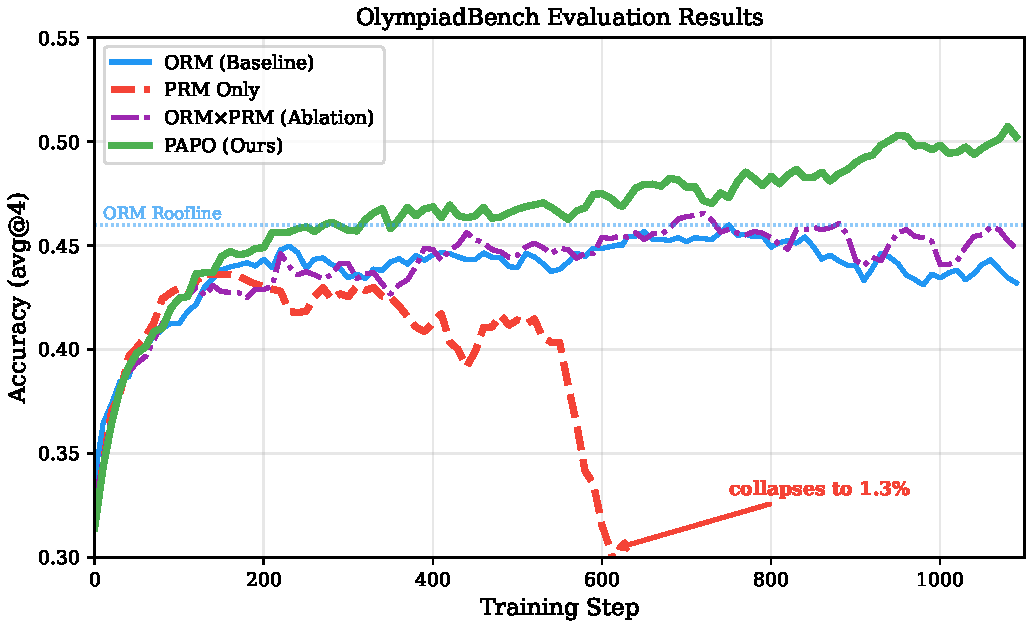
\includegraphics[width=\textwidth]{figures/fig_training_curves.pdf}
    \caption{OlympiadBench evaluation results.}
    \label{fig:hero-a}
\end{subfigure}
\hfill
\begin{subfigure}[b]{0.42\textwidth}
    \centering
    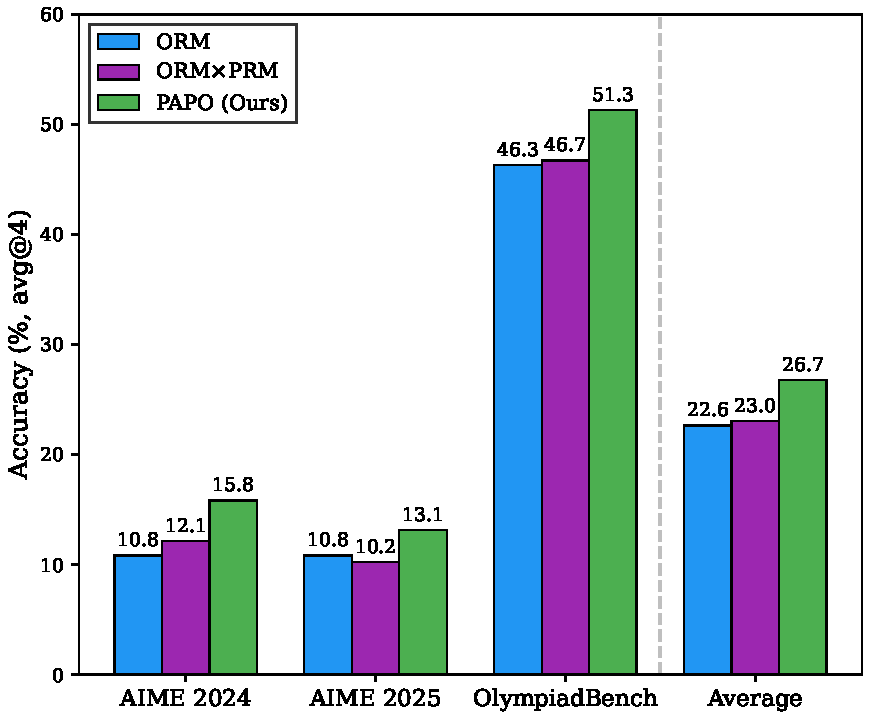
\includegraphics[width=\textwidth]{figures/fig_hero_panel_b.pdf}
    \caption{Accuracy on competition math.}
    \label{fig:hero-b}
\end{subfigure}
\caption{\textbf{(a)} ORM (blue) plateaus and declines after step 750 due to signal exhaustion; PRM (red, dashed) collapses via reward hacking; ORM$\times$PRM (purple, dash-dotted) tracks ORM closely without exceeding it; \method{} (green) continues improving throughout training, reaching 51.3\%. \textbf{(b)} Comparison across AIME 2024/2025, OlympiadBench, and their average. Naive multiplicative combination (ORM$\times$PRM) barely improves over ORM, while \method{}'s decoupled normalization yields substantial gains on all benchmarks.}
\label{fig:hero}
\end{figure*}

To solve this problem, we propose \textbf{Process-Aware Policy Optimization (\method{})}, which integrates rubric-based process evaluation into GRPO through \textbf{decoupled advantage normalization}. \method{} constructs the advantage from two independently normalized components:
\begin{itemize}
    \item An \textbf{outcome advantage} $\aout$, computed from binary ORM rewards via standard GRPO normalization, anchoring the training signal on answer correctness.
    \item A \textbf{process advantage} $\aproc$, computed from rubric-based PRM scores normalized \emph{exclusively among correct responses}, differentiating reasoning quality within the correct group.
\end{itemize}
This decoupled formulation mitigates reward hacking by separating PRM-based reasoning rewards from the final-answer signal. As a result, $\aproc$ can still provide non-zero gradients even when all responses are correct. Importantly, normalization is performed only over correct responses, ensuring that PRM scores do not distort the outcome signal and that incorrect responses are not rewarded solely for strong reasoning traces.

As shown in Figure~\ref{fig:hero}a, \method{} continues improving throughout training, reaching 51.3\% on OlympiadBench \citep{he2024olympiadbench} while ORM peaks at 46.3\% and declines, and Figure~\ref{fig:hero}b shows that the improvement generalizes to other math competition benchmarks like AIME \citep{balunovic_srimatharena_2025}.

To summarize, our contributions are as follows:
\begin{enumerate}
    \item We identify a dilemma in GRPO reward design: binary ORM lacks process supervision and suffers from signal exhaustion, yet naively using PRM scores causes reward hacking and training collapse.
    \item We propose \method{}, which composes the advantage from independently normalized outcome and process components with correct-subset normalization, resolving this dilemma.
    \item We show that \method{} consistently outperforms ORM across model scales from 3B to 14B and six benchmarks, including larger models where ORM is already strong.
\end{enumerate}
